%%%%%%%%%%%%%%%%%%%%%%%%%%%%%%%%%%%%%%%%%%%%%%%%%%%%%%%%%%%%%%%%%%%%%%%%
%%% LaTeX Template for AAMAS-2026 (based on sample-sigconf.tex)
%%% Prepared by the AAMAS-2026 Publication Chairs based on the version from AAMAS-2025.
%%%%%%%%%%%%%%%%%%%%%%%%%%%%%%%%%%%%%%%%%%%%%%%%%%%%%%%%%%%%%%%%%%%%%%%%

% --------------------------------------------------------------------
% Document class
% --------------------------------------------------------------------
%%% == IMPORTANT ==
%%% Use the first variant below for the final paper (including author information).
%%% Use the second variant below to anonymize your submission (no author information shown).
%%% For further information on anonymity and double-blind reviewing,
%%% please consult the call for paper information:
%%% https://cyprusconferences.org/aamas2026/submission-instructions/

%%%% For anonymized submission, use this:
%\documentclass[sigconf,anonymous]{acm/aamas}

%%%% For camera-ready, use this:
% \documentclass[sigconf]{acm/aamas}
\documentclass[manuscript]{acm/aamas}

% --------------------------------------------------------------------
% Core packages (many already included by aamas class)
% --------------------------------------------------------------------
\usepackage{balance}      % balance columns on the final page
\usepackage{algorithm}    % algorithm environment
\usepackage{algorithmic}  % algorithmic typesetting
\usepackage{float}        % improved float placement control
\usepackage{tikz}         % graphics and diagrams
\usetikzlibrary{positioning,shapes,arrows,shadows,fit}
\usepackage{ctable}       % complex table formatting
\usepackage{array}        % extended array and tabular
\usepackage{ulem}         % underlining and strikethrough
\usepackage{ragged2e}     % improved ragged text alignment

% Custom column type for right-aligned paragraph columns
\newcolumntype{R}[1]{>{\raggedleft\arraybackslash}p{#1}}

% --------------------------------------------------------------------
% AAMAS-2026 copyright block (DO NOT CHANGE!)
% --------------------------------------------------------------------
\setcopyright{ifaamas}
\acmConference[AAMAS '26]{Proc.\@ of the 25th International Conference
on Autonomous Agents and Multiagent Systems (AAMAS 2026)}{May 25 -- 29, 2026}
{Paphos, Cyprus}{C.~Amato, L.~Dennis, V.~Mascardi, J.~Thangarajah (eds.)}
\copyrightyear{2026}
\acmYear{2026}
\acmDOI{}
\acmPrice{}
\acmISBN{}

\definecolor{Orange}{rgb}{1,0.5,0}
\definecolor{Purple}{rgb}{1,0,1}
\definecolor{Gray}{rgb}{0.6,0.6,0.6}
\definecolor{Green}{rgb}{0.1,0.6,0.1}
\definecolor{Teal}{rgb}{0.0, 0.55, 0.55}
\definecolor{Pink}{rgb}{1, 0.4, 0.6}
\definecolor{Blue}{rgb}{0,0,1}

\newcommand{\todo}[1]{\textsf{\textbf{\small \textcolor{Purple}{[[#1]]}}}}
\newcommand{\todoname}[3]{ \textcolor{#1}{\textsf{\textbf{\small [[#2 says: #3]]}}}}
\newcommand{\kb}[1]{\todoname{Orange}{Kevin}{#1}}
\newcommand{\gsh}[1]{\todoname{Green}{Galen}{#1}}
\newcommand{\samarth}[1]{\todoname{Blue}{Samarth}{#1}}
\newcommand{\anil}[1]{\textcolor{blue}{#1}}
\newcommand{\mlwcomment}[1]{\textcolor{blue}{MLW: #1}}
\newcommand{\adscomment}[1]{\textcolor{Orange}{Aaron: #1}}
\newcommand{\tool}{MEKH}
\newcommand{\toolname}{Material Evolution Knowledge Hypergraph}
\newcommand{\process}{MP-DNF}
\newcommand{\processname}{Material Processing Dependency Network Framework}
\newcommand{\Hcal}{\mathcal{H}}

% --------------------------------------------------------------------
% Submission information
% --------------------------------------------------------------------
%%% == IMPORTANT ==
%%% Use this command to specify your submission number.
%%% In anonymous mode, it will be printed on the first page.
\acmSubmissionID{1162}

% --------------------------------------------------------------------
% Cover page configuration (internal use only)
% --------------------------------------------------------------------
% Load geometry only when cover is enabled (may conflict with ACM class)
\newif\ifusecoverpage
\usecoverpagetrue              % set \usecoverpagefalse to skip cover

\ifusecoverpage
  \usepackage{geometry}        % temporary margin adjustments for cover
\fi

\usepackage{fancyhdr}          % custom page styles
\usepackage{xcolor}            % color support for branding

% Brand color for cover page footer
\definecolor{uvaorange}{RGB}{232,119,34}

% Define the 'trcover' pagestyle (logo + footer text)
\input{coverpage/coverpage_style}

% --------------------------------------------------------------------
% Author data and venue-specific formatting
% --------------------------------------------------------------------
% Centralized author database: defines \AllAuthorData and stub \OneAuthor
\input{authors_db}

% Per-paper selection: comma-separated list of author IDs, no spaces
% Authors will appear in the order specified here
\newcommand{\SelectedAuthors}{1,2,3,4,5,6,7,8,9,10,11}

% ACM/AAMAS-specific author/affiliation formatting
% Defines \acmauthors using \AllAuthorData + \SelectedAuthors
\input{acm/formats_acm}

% --------------------------------------------------------------------
% Title and author metadata
% --------------------------------------------------------------------
\newcommand{\PaperTitle}{%
  An Agentic AI Approach for Material Evolution Knowledge Hypergraph Discovery%
}

\title{\PaperTitle}

% Populate ACM author and affiliation metadata from shared data
\acmauthors

% --------------------------------------------------------------------
% Abstract and executive summary (to be filled by authors)
% --------------------------------------------------------------------
% Use this environment for the ACM/AAMAS abstract that appears under the title.
% Keep it focused on the research contribution, methods, and key results.
\newcommand{\PaperAbstract}{%
Supply chain analysis for critical materials often employs top-down methods, tracing backward from finished products. These methods can lack visibility into intermediate dependencies due to proprietary manufacturing and opaque supplier networks. This paper presents a bottom-up agentic AI approach for constructing a ~\toolname{} (\tool{}), an essential building block for supply chain networks that document the transformation of raw materials into advanced technological products.

The approach uses the \processname{} (\process{}), a multi-agent system in which specialized language models iteratively discover, classify, and validate materials and industrial processes. Multiple knowledge sources are integrated via the Model Context Protocol (MCP), including harmonized trade code databases, semantic reference caches, web searches, and structured encyclopedic sources. The resulting networks are represented as directed hypergraphs that capture the multi-input, multi-output nature of industrial processes.

The pipeline begins with seed materials and expands through a documented process, identifying intermediates and transformations, and applying validation based on reference quality. Iterative cycles allow the introduction of new materials, process discovery, validation, and the removal of weakly supported links. A key feature is the explicit identification and tracking of material derivatives, which can be refined in different countries and assigned a unique, harmonized shipping code, supporting more precise supply chain tracking.

Technical contributions include: formalizing supply chain transformations using directed hypergraphs; enabling iterative bottom-up network discovery; deploying LLM agents for scalable extraction and validation; and referencing all process steps for traceability and assessment.

This framework supports mineral pathway analysis, bottleneck detection, and supply chain resilience by revealing alternatives and dependencies that are not readily apparent in top-down mapping. The pipeline, managed through a modular command-line interface, is suited to both research and operational supply chain analysis and construction.
}

% Use this macro for the internal report executive summary used on the cover page
% and possibly in an introductory section. Aim at senior leadership and analysts.
\newcommand{\ExecutiveSummary}{%
This work introduces a bottom‑up AI framework that maps how raw minerals move through industrial processes to become advanced technologies, providing visibility that traditional top‑down supply chain methods often miss. Instead of relying solely on opaque supplier networks, specialized AI agents systematically discover and validate materials, transformation steps, and intermediate products using multiple trusted data sources. The resulting hypergraph networks expose critical pathways, derivatives, and chokepoints, enabling analysts to spot vulnerabilities, alternative routes, and opportunities for resilience that are not obvious from finished‑product data alone. Delivered as a modular command‑line tool, the system is designed for both research and operational use in mineral pathway analysis, bottleneck detection, and strategic supply chain planning.
}

% ====================================================================
% Document body
% ====================================================================
\begin{document}

% Coverpage (internal use only; comment out for submission)
\ifusecoverpage
  \input{coverpage/insert_coverpage}
\fi

%%% The following commands remove the headers in your paper. For final
%%% papers, these will be inserted during the pagination process.

\pagestyle{fancy}
\fancyhead{}


% Abstract section using the placeholder macro
\begin{abstract}
\PaperAbstract
\end{abstract}

% Construct title section
\maketitle

%%%%%%%%%%%%%%%%%%%%%%%%%%%%%%%%%%%%%%%%%%%%%%%%%%%%%%%%%%%%%%%%%%%%%%%%

\section{Introduction}
\label{sec:introduction}

Modern industrial ecosystems rely on complex, multistage transformations that convert naturally occurring raw materials into intermediate chemicals and ultimately into advanced technological products. Understanding the pathways connecting raw material extraction to refined intermediates and high-value products is crucial for identifying vulnerable dependencies in global supply chains, assessing critical mineral risks, and discovering alternative production routes during disruptions.

Traditional supply chain analysis predominantly employs top-down approaches that trace backward from finished products through supplier networks. However, these methods face significant limitations due to opaque supplier networks and proprietary manufacturing processes that obscure intermediate dependencies~\cite{colon2022systemic}. Recent real-world disruptions have demonstrated the critical consequences of these analytical blind spots~\cite{hasan2022demand, chakraborty2022empirical, tam2022understanding}.

Such dependencies can be studied more systematically through knowledge graph (KG) representations.
KGs have been constructed in various domains, including medicine~\cite{brbic2024predicting}, biology, and material sciences~\cite{venugopal2024matkg, mrdjenovich2020propnet}.
For instance, knowledge graphs in material sciences~\cite{venugopal2024matkg}, extract relationships between 
the complete space of materials and their properties and applications, processes and methods for synthesis, and other characteristics.
These provide a systematic approach to organizing scientific data and allow researchers to analyze and understand material science datasets, and discover new types of processes and materials.
Until recently, such knowledge graphs were extracted automatically using standard natural language processing methods, from well-structured scientific publications~\cite{Stocker2023Creating, Dessi2021Generating}.

However, KG construction is more difficult in the case of supply chain networks for multiple reasons. 
First, material classes are less structured, as they include inputs for diverse contexts, such as industry, not just laboratories.
Second, data is available in a broad range of documents, including public literature, patents, and technical references, in addition to scientific publications.
Therefore, a new class of KGs are needed to provide a foundation for evidence-based network construction that avoids the opacity constraints of top-down approaches.
Finally, graph representations are insufficient for many of these processes, as they involve transforming a set of inputs into a set of outputs, and non-binary relations must be considered.
A hypergraph representation is more suitable for such information, and has been proposed in the literature \cite{wolf2016advantages, fatemi2019knowledge, luo2025hypergraphrag}.
Wolf et al.~\cite{wolf2016advantages} show that ``hypergraphs better model complex, non-pairwise relationships, are computationally more efficient, and can represent temporal and locality effects, unlike binary graphs''. Luo et al.~\cite{luo2025hypergraphrag} demonstrate that hypergraph knowledge representation provides ``knowledge completeness, structural expressiveness, and inferential capability'' superior to binary graph approaches.
Fatemi et al.~\cite{fatemi2019knowledge} show that knowledge hypergraphs are a solution to the problem that traditional binary knowledge graphs cannot adequately represent relations involving more than two entities, even though over one-third of entities in real-world knowledge bases participate in such non-binary relations. While some previous research has been conducted separately applying knowledge graph theory~\cite{kosasih2022towards, almahri2024enhancing} and hypergraph approaches to the mapping of supply-chains~\cite{suo2018exploring, li2023research}, an approach utilizing knowledge hypergraphs (KHGs) has not yet been developed.

%Knowledge hypergraphs have not been developed for supply chain networks, especially using diverse kinds of unstructured datasets which contain such information. 
%\anil{some more discussion, citations}

% In contrast, a bottom-up approach begins with naturally occurring materials and systematically follows documented industrial transformations to construct complete transformation networks. This methodology leverages the fact that upstream industrial processes are often well-documented in public literature, patents, and technical references, providing a foundation for evidence-based network construction that avoids the opacity constraints of top-down approaches.



% This paper presents a bottom-up agentic AI approach for constructing 
% % \textbf{Material Evolution Graphs} (MEGs). 
% \emph{Material Evolution Knowledge Hypergraph} (\tool{}).
% A Material Evolution Graph (MEG) \mlwcomment{This looks weird, defining two different terms as "MEG" (especially since one of them does not abbreviate to MEG). We should be consistent in our terminology and only use MEG for one term (and ideally only define it once -- yesterday "MEG" was defined multiple times.)} maps material transformation pathways from naturally occurring forms (ores, mineral compounds, and brines) through 
% processing stages to their eventual form for use in technological products. The MEG serves as the foundational component for constructing a full \sout{\textbf{Technology Dependency Network} (TDN)} supply chain network that systematically maps industrial transformation pathways from naturally occurring raw materials through to their eventual use in the manufacture of advanced technological products. \samarth{Maybe we should avoid discussion of TDNs here, since we don't have a published paper we can point to.}. \adscomment{It used to all say TDN. Was trying to massage it. I agree, probably don't want TDN, but will need to say what it is used for.} \sout{A TDN is a multi-level, hierarchical representation that systematically delineates the interdependencies underpinning the development and maintenance of a specific technology. Formally, we define a TDN as a directed acyclic multipartite relational graph $G(V, E)$ with known levels $L_1, L_2, \ldots, L_k$, where each level represents a separate dependency tier ranging from complete technologies to components, materials, and producing countries. Vertices are formed as a union of subsets of $L_1, \ldots, L_k$, with edges connecting lower levels to higher levels: $\bigcup_{i=1}^{k-1} L_i \times L_{i+1}$. Each edge has weight $w_{uv} > 0$ indicating the influence input $u$ has on production of $v$. For country-to-material edges, weights represent production proportions.}

\noindent
\textbf{Our Contributions.}\\
(1) We present a bottom-up agentic AI approach for constructing a 
\emph{Material Evolution Knowledge Hypergraph} (\tool{}), a labeled directed multi hypergraph for representing how material transformation processes transform a set of inputs to outputs through 
processing stages to their eventual form for use in technological products.
Such information cannot be represented through standard knowledge graphs~\cite{venugopal2024matkg, mrdjenovich2020propnet}.
\tool{} serves as the foundational component for constructing a full  supply chain network that systematically maps industrial transformation pathways from naturally occurring raw materials through to their eventual use in the manufacture of advanced technological products. We refer to the process of building an MEKH as the \processname{} (\process{}).

\iffalse
\begin{figure}[h]
    \centering
    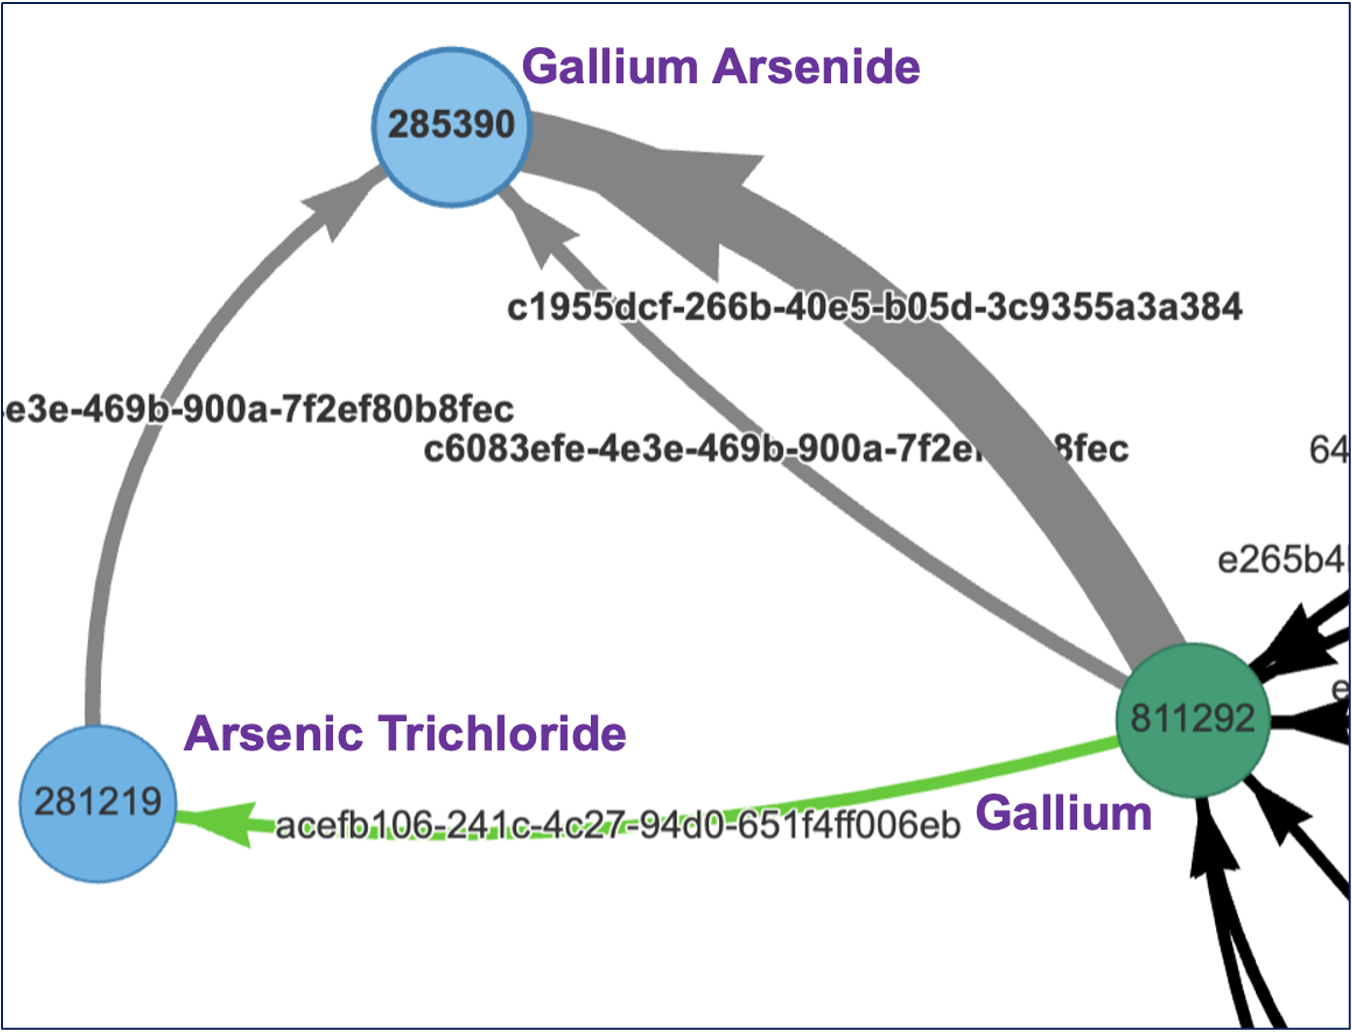
\includegraphics[width=0.9\linewidth]{images/gallium-arsenide.png}
    \caption{Partial \tool{} showing example relationships between a mineral and multiple compounds, each with a different assigned HS Shipping Code. \samarth{We need some more detail. Perhaps a visualization of the whole network, with this bit shown in an inset?} \samarth{actually, given Fig.~\ref{fig:pipeline}, do we need this one?}
    \adscomment{I was just trying to provide a visual to break-up a long text section. With Fig 4, probably don't need.} \mlwcomment{If we do keep, probably need a legend}}
    \label{fig:pipeline}
\end{figure}
\fi


\iffalse
We employ a multi-agent architecture in which specialized LLM agents discover, classify, and validate materials and industrial processes. 
By representing supply chains as directed hypergraphs that accommodate multi-input, multi-output industrial processes, the system constructs traceable, evidence-backed networks that reveal transformation pathways from naturally occurring materials to advanced technological products.
\anil{some overlap with earlier para}
\fi


\process{} involves an iterative, bottom-up discovery.
The pipeline begins with raw inputs and expands through multiple 
iterations to cover entire transformation chains, uncovering intermediates that are invisible in top-down analyses.
We develop tools for LLM-assisted reasoning for scalable knowledge extraction, where specialized agents discover, classify, and validate materials and processes from unstructured references. 
Each transformation edge is supported by multiple references, scored for source quality and content relevance, enabling trustworthy networks, providing 
evidence-backed process validation.

\noindent
(2) We use our approach to construct \tool{}s for some of the critical minerals used in microelectronics, for example, Boron.
\tool{} identifies all key routes from ore to advanced compounds.
We analyze structural properties of these hypergraphs, and notions of criticality of materials involved. 
This can guide supply chain resilience planning, and can reveal alternative routes for strategic materials.

% \noindent
% \textbf{Contributions:} 
% \samarth{need to expand and itemize; we have multiple contributions}
% \sout{The key contribution of this work lies in demonstrating how agentic AI systems can overcome the fundamental limitations of traditional supply chain analysis by systematically constructing bottom-up material transformation networks. Unlike top-down approaches that encounter opacity barriers, or manually curated knowledge graphs that lack scalability, this automated approach scales to complex industrial networks while maintaining traceability to verifiable sources. The resulting networks enable critical mineral pathway analysis, bottleneck identification, and supply chain resilience planning by revealing alternative production routes and intermediate dependencies that remain hidden in conventional analyses.}

% This pipeline contributes several key innovations:

% \begin{enumerate}
%     \item We formalize supply chain transformations as a directed hypergraph. This naturally represents 
%     realistic processes with multi-input, multi-output structures, unlike simple graph models.
%     \item Iterative, bottom-up discovery: the pipeline begins with raw inputs and expands through multiple 
%     iterations to cover entire transformation chains, uncovering intermediates that are invisible in top-down 
%     analyses.
%     \item LLM-assisted reasoning for scalable knowledge extraction: Specialized agents discover, classify, and validate materials and processes from unstructured references.
%     \item Evidence-backed process validation: Each transformation edge is supported by multiple references, scored for source quality and content relevance, enabling trustworthy networks.
% \end{enumerate}

% This work enables:

% \begin{itemize}
%     \item Critical mineral pathway analysis—understanding all possible routes from ore to advanced compounds.
%     \item Identification of bottlenecks—finding intermediate compounds that connect multiple downstream technologies.
%     \item Supply chain resilience planning—revealing alternative routes for strategic materials.
% \end{itemize}
\section{Related Work}
\label{sec:related}

The construction of \toolname{}s through bottom-up processes intersects several established research domains, particularly multi-agent systems, knowledge graph construction, and supply chain modeling.

\textbf{Multi-Agent Systems for Supply Chain Management.} 
Multi-agent systems have been applied to supply chain management to address distributed decision-making and coordination challenges. Jaimez-González and Luna-Ramírez~\cite{jaimez2021towards} proposed a multi-agent architecture for supply chain management that employs specialized agents for different operational functions, demonstrating how agent-based approaches can handle complex coordination tasks. They demonstrate using specialized agents in supply chain contexts, though their focus remains on operational management rather than network discovery. More recently, Farazi~\cite{farazi2025enhancing} examined multi-agent systems combined with machine learning for supply chain resilience, showing how agent coordination can support adaptive responses to disruptions. We apply specialized LLM agents specifically for knowledge extraction and network construction rather than operational coordination.

% What part is "automomous"? -constructing an optimal supply chain?
Research on autonomous supply chains has further developed multi-agent frameworks for supply chain automation~\cite{santos2024implementing, vanderheijden2024multiagent}. These studies demonstrate agent-based coordination for supply chain operations but do not address the fundamental problem of network discovery and material transformation mapping that our approach tackles. Our contribution differs by focusing agents on iterative knowledge discovery rather than operational execution.

\textbf{Knowledge Graphs and Supply Chain Analysis.} 
Knowledge graph construction for supply chain management has received increased attention as organizations seek better visibility into complex networks. AlMahri et al.~\cite{almahri2024enhancing} demonstrated how knowledge graphs combined with large language models can support supply chain visibility through automated information extraction from unstructured sources. They extract entity relationships from existing documentation. 
While this work provides relevant methodology, it does not construct 
material transformation networks from naturally occurring materials. Liu et al.~\cite{liu2025designing} developed a knowledge-enhanced framework for supply chain information integration that shows how structured knowledge representations can support complex supply chain analysis. While their work focuses on integrating existing supply chain data, our approach addresses the prior challenge of discovering and constructing the underlying transformation networks.

Zhao et al.~\cite{zhao2024systematic} identify challenges of automated knowledge extraction from heterogeneous sources, which directly relates to our approach of using multiple knowledge sources through the Model Context Protocol to construct material evolution graphs.

\textbf{Hypergraph Models for Complex Systems.} 
Traditional graph representations have limitations when modeling systems with multi-input, multi-output relationships. Recent work on hypergraph models for enterprise supply chain networks~\cite{li2024research} demonstrates how hypergraph structures can capture complex relationships that exceed the capabilities of standard directed graphs. Li et al. show the representation of supply chain relationships as hypergraphs but focus on enterprise-level network modeling rather than material transformation processes. Our approach extends hypergraph applications to material-level transformations where industrial processes naturally involve multiple inputs producing multiple outputs.

Graph neural networks for supply chain analytics have also explored advanced graph structures~\cite{zhang2024graph}, showing how sophisticated graph representations can support complex supply chain analysis tasks. Graph neural network research offers relevant methods for our hypergraph representation but do not address the specific challenges of material transformation network construction.

\textbf{Bottom-Up Network Construction Approaches.} 
Bottom-up approaches to supply chain modeling have been explored in various contexts. Shapiro~\cite{shapiro1998bottom} provided foundational analysis comparing bottom-up versus top-down approaches to supply chain management, demonstrating that bottom-up methods can reveal system-level properties that top-down approaches miss. This theoretical foundation supports our approach but does not address the computational challenges of automated bottom-up network construction. More recent work by Yang et al.~\cite{yang2023integrating} applied bottom-up modeling to building material networks, showing how starting from base materials and following transformation processes can construct comprehensive networks. Their work validates the bottom-up approach for material systems but focuses on construction materials rather than broader industrial transformation networks.

The limitations of top-down supply chain analysis have been empirically demonstrated by Baldwin et al.~\cite{baldwin2023hidden}, who showed that conventional backward-tracing approaches significantly underestimate supply chain dependencies due to hidden intermediates. Their findings provide empirical justification for bottom-up approaches but do not propose computational solutions for automated network construction.

\textbf{Research Gaps and Positioning.} 
Existing approaches to supply chain network construction remain largely manual and do not scale to comprehensive material transformation mapping. We address this limitation through specialized LLM agents that discover and validate material transformations iteratively. Prior work has not combined multi-agent systems with knowledge graph construction, and specifically knowledge hypergraph construction, for bottom-up material network discovery.
\section{Method/Approach}
\label{sec:method}

\subsection{Formal Definition}

We formally define a \emph{Material Evolution Knowledge Hypergraph} (\tool{}) as a directed labeled multi-hypergraph $\Hcal(M, E)$ \cite{ouvrardHypergraphsIntroductionReview2020}, where $M$ and $E$ denote a set of materials (also referred to as nodes) and the set of directed hyper-edges, respectively. 
Each (directed) hyper-edge $e=(e_s, e_t)\in E$ corresponds to a chemical or industrial \textit{process} $\mathbf{P_e}$, which transforms a set $e_s=\{m_1, \ldots m_p\}\subset M$ of inputs to a set $e_t=\{m_q, \ldots, m_r\}\subset M$ of outputs.
We refer to $e_s, e_t$ as the source and target of $e$, respectively.
% the process corresponding to $e$ transforms the source set $e_s =\{m_1, \ldots m_p\}$ of materials (the inputs of the process) to the target set $e_t=\{m_q, \ldots, m_r\}$ (the outputs of the process).
% the source $e_s$ is a \textit{process}, that uses as inputs a set of materials $m_1, \ldots m_p \in M$, and produces a set of outputs $m_q, \ldots, m_r \in M$.
%Each process requires a specific set of inputs, and produces a specific set of outputs. 
% \samarth{need to write in a more complete and formal manner}  
We use $\ell(e)=\mathbf{P}_e$ as the label for the hyperedge $e$.
There could be multiple processes $\mathbf{P}_{e_1}, \mathbf{P}_{e_k}$ transforming a source set $S$ to a target set $T$;
these would be represented as multiple hyper-edges $e_i=(S, T)$ with $\ell(e_i)=\mathbf{P}_{e_i}$.

We focus on the set $M$ of materials in the Harmonized System (which is a standardized numerical method of classifying traded products); all such materials have a valid Harmonized System (HS) Codes~\cite{hscode}.
We focus here on 6-digit HS codes, which represent aggregations of many products.

Our algorithm for producing ~\tool s is presented in Algorithm \ref{alg:tdn-pipeline}.
The ProcessGeneration method referred to in this Algorithm is a strategy that queries auxiliary resources $A$ to find processes, and filters the results based on several quality and relevance metrics. 

% OLD ALGORITH
\iffalse
\begin{algorithm}[h]
\caption{Bottom-Up Material Evolution Graph (System Process Overview) \samarth{rewrite using hypergraph terminology, expand lines 4,5,6}}
\label{alg:tdn-pipeline}
\begin{algorithmic}[1]

{\color{gray}
\REQUIRE number of iterations $n$, seed materials $s$, auxiliary data $A$, universe of allowable materials $\mathcal{M}$
\STATE $\text{Processes} \gets \emptyset$
\STATE $\text{Materials} \gets s$

\FOR{$i = 1, \ldots, n$}
    \STATE Update Processes from $\text{ProcessGeneration}(\text{Materials}, A)$
    \STATE Each process has a set of inputs, outputs $p_{in}, p_{out} \subset \mathcal{M}$
    \STATE Update Materials with $p_{in} \cup p_{out}$ for each new process
\ENDFOR
\RETURN $MEG = (\text{Materials}, \text{Processes})$ 
}
\end{algorithmic}
\end{algorithm}
\fi

% NEW ALGORITHM USING HYPEREDGE TERMS
\begin{algorithm}[h]
\caption{Bottom-Up \toolname (System Process Overview)} 
%\adscomment{Does this work/make sense as replacement?}
\label{alg:tdn-pipeline}
\begin{algorithmic}[1]
\REQUIRE number of iterations $n$, seed vertex set (seed materials) $s$, auxiliary hypergraph data $A$, universe of allowable vertices (materials) $\mathcal{V}$
\STATE $\text{Hyperedges (Processes)} \gets \emptyset$
\STATE $\text{Vertices (Materials)} \gets s$

\FOR{$i = 1, \ldots, n$}
    \STATE Update Hyperedges from $\text{ProcessGeneration}(\text{Vertices}, V)$
    \STATE Each hyperedge has a set of inputs, outputs e_{in}, e_{out} \subset \mathcal{V}$
    \STATE Update Vertices with $e_{in} \cup e_{out}$ for each new process
\ENDFOR
\RETURN $MEKH = (\text{Vertices}, \text{Hyperedges})$ 

\end{algorithmic}
\end{algorithm}

\subsection{Rationale}
The system architecture incorporates several design principles that address the requirements of industrial supply chain modeling. The directed hypergraph representation accommodates the multi-input, multi-output structure that characterizes industrial processes, providing a mathematical foundation that captures transformation complexity. The iterative pipeline methodology supports systematic network growth through discrete expansion cycles, maintaining traceability to source evidence and quality control through validation mechanisms at each stage. Integration with the Model Context Protocol enables LLM agents to access specialized tools and knowledge sources, thereby enhancing their reasoning capabilities and evidence retrieval processes while maintaining modularity. The command-line interface provides reproducible control over the pipeline workflow, supporting both research applications and operational supply chain analysis through user-directed network construction and inspection capabilities.

\subsection{Architectural Layers}
The bottom-up supply chain pipeline is built around a modular, iterative architecture designed to progressively construct a material evolution graph — a representation of how raw materials are transformed into intermediates for use in advanced products through industrial processes. The architecture consists of three interdependent layers that collectively support data representation, knowledge discovery, and user interaction.

\begin{figure}[htbp]
\centering
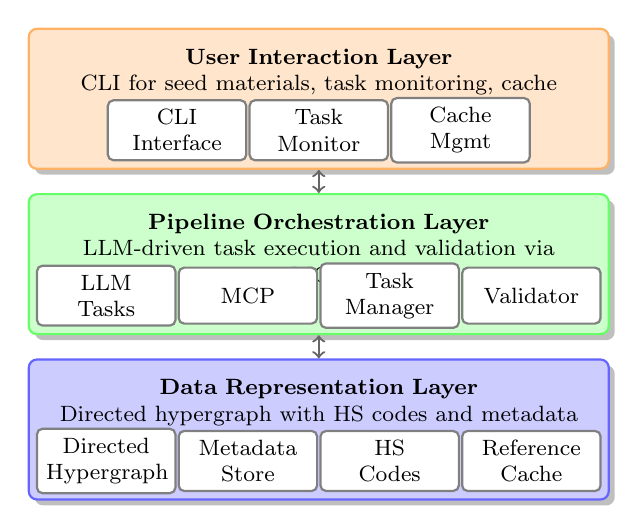
\begin{tikzpicture}[
    layer/.style={
        rectangle, rounded corners=3pt,
        minimum width=2.9in, minimum height=0.7in,
        text width=2.7in, align=center,
        font=\footnotesize, drop shadow
    },
    data/.style={layer, fill=blue!20, draw=blue!60, thick},
    orchestration/.style={layer, fill=green!20, draw=green!60, thick},
    interface/.style={layer, fill=orange!20, draw=orange!60, thick},
    component/.style={
        rectangle, rounded corners=2pt,
        minimum width=0.65in, minimum height=0.28in,
        text width=0.6in, align=center,
        font=\footnotesize, fill=white, draw=black!50, thick
    },
    arrow/.style={->, thick, draw=black!60},
    link/.style={thin, draw=gray!60}
]

% Layers (top to bottom)
\node[interface] (ui_layer) at (0,5.0) {
    {\begin{minipage}[t][0.5in][t]{2.6in}
      \centering
      \textbf{User Interaction Layer}\\
      CLI for seed materials, task monitoring, cache management
    \end{minipage}}
};

\node[orchestration] (orch_layer) at (0,2.9) {
    {\begin{minipage}[t][0.5in][t]{2.6in}
      \centering
      \textbf{Pipeline Orchestration Layer}\\
      LLM-driven task execution and validation via MCP
    \end{minipage}}
};

\node[data] (data_layer) at (0, 0.8) {
    {\begin{minipage}[t][0.5in][t]{2.6in}
      \centering
      \textbf{Data Representation Layer}\\
      Directed hypergraph with HS codes and metadata
    \end{minipage}}
};

% Components (kept clear of layer text)
\node[component] (cli)      at (-1.8,4.6) {CLI\\Interface};
\node[component] (monitor)  at (0,4.6)    {Task\\Monitor};
\node[component] (cache)    at (1.8,4.6)  {Cache\\Mgmt};

\node[component] (llm)       at (-2.7,2.5) {LLM\\Tasks};
\node[component] (mcp)       at (-0.9,2.5) {MCP};
\node[component] (manager)   at (0.9,2.5)  {Task\\Manager};
\node[component] (validator) at (2.7,2.5)  {Validator};

\node[component] (hypergraph) at (-2.7,0.4) {Directed\\Hypergraph};
\node[component] (meta)       at (-0.9,0.4) {Metadata\\Store};
\node[component] (hs)         at (0.9,0.4)  {HS\\Codes};
\node[component] (cache2)     at (2.7,0.4)  {Reference\\Cache};

% Inter-layer relations
\draw[<->, thick, draw=black!60] (ui_layer.south) -- (orch_layer.north);
\draw[<->, thick, draw=black!60] (orch_layer.south) -- (data_layer.north);

\end{tikzpicture}
\caption{Architectural Layers and Related Tools of the Bottom-Up Supply Chain Pipeline. %\samarth{Can we increase the font size
%in the white boxes?}
}
\end{figure}

\textbf{Data Representation Layer.}
The data representation layer defines the structure of the supply chain network as a directed hypergraph. This framework captures the complexity of industrial processes, including scenarios where several materials are inputs to a process and multiple outputs are possible. Additional metadata, such as harmonized system (HS) codes, process references, and a reference cache, are recorded to support semantic searches and detailed reasoning.

\textbf{Pipeline Orchestration Layer.}
The orchestration layer manages the execution of tasks that develop and refine the material evolution graph. These tasks—adding new materials, identifying process relationships, merging duplicate entries, and validating references—are assigned according to their function. Many are driven by large language models using resources and search tools configured through the Model Context Protocol.

\textbf{User Interaction Layer.}
Interaction with the pipeline is handled through a command-line interface. This interface allows users to provide seed materials, initiate or monitor expansion and validation tasks, maintain the reference cache, and review the current state of the evolving network. Each architectural layer operates independently; for example, the data layer can be updated with new sources without changes to orchestration or interface logic.

Each layer is designed for independent modification and extension; for instance, data sources can be updated without altering orchestration or interface logic.


\iffalse
\subsection{System Workflow}
The general workflow supports the automated discovery and interactive refinement of \toolname{}s, enabling control over both the scope of exploration and the level of detail achieved. The following sequence outlines the main steps involved in configuring and operating the \toolname{} construction pipeline. Many of the steps in the workflow are completed with the aid of one or more LLM agents. These agents are described in the System Pipeline and Agents section below.

\begin{enumerate}
\item The user sets up a research context using the command-line interface and specifies a primary seed material to begin network construction. Additional optional inputs may include specific intermediate material forms, reference documents for initial evidence, and a list of product families to guide downstream expansion.

\item If no optional configuration is provided, the pipeline begins with the seed material and incrementally identifies relevant materials and processes from that starting point.

\item The system performs a sequence of tasks: it expands the material set, identifies relevant industrial processes, collects and evaluates references, and removes unsupported connections in the network.

\item With each iteration, newly identified materials enable process mapping and downstream expansion. Material and process relationships are refined, with ongoing validation and traceability to supporting evidence.

\item The reference cache is updated as the workflow proceeds and indexed to support semantic search. Accumulated data and references from past iterations are used to inform subsequent expansions and validations.

\item The user may pause the workflow to review progress or modify parameters by adding materials or references, then resume network construction from the current state.

\end{enumerate}
\fi


\subsection {System Pipeline \& Agents}
The general workflow, as seen in figure \ref{fig:pipeline}, supports the automated discovery and interactive refinement of \toolname{}s, enabling control over both the scope of exploration and the level of detail achieved.
The implementation of the pipeline is organized into discrete, composable tasks, each responsible for a specific part of network expansion or refinement. These tasks can run independently or be combined into a complete iterative workflow. Many tasks rely on \textbf{task-specific LLM agents} that have access to structured auxiliary data and semantic search tools. There are currently 6 task-specific agents utilized in the pipeline: material classification agent, material finder agent, material manufacturing agent, process merging agent, reference reviewer agent, and url scorer agent.

\begin{figure}[h]
    \centering
    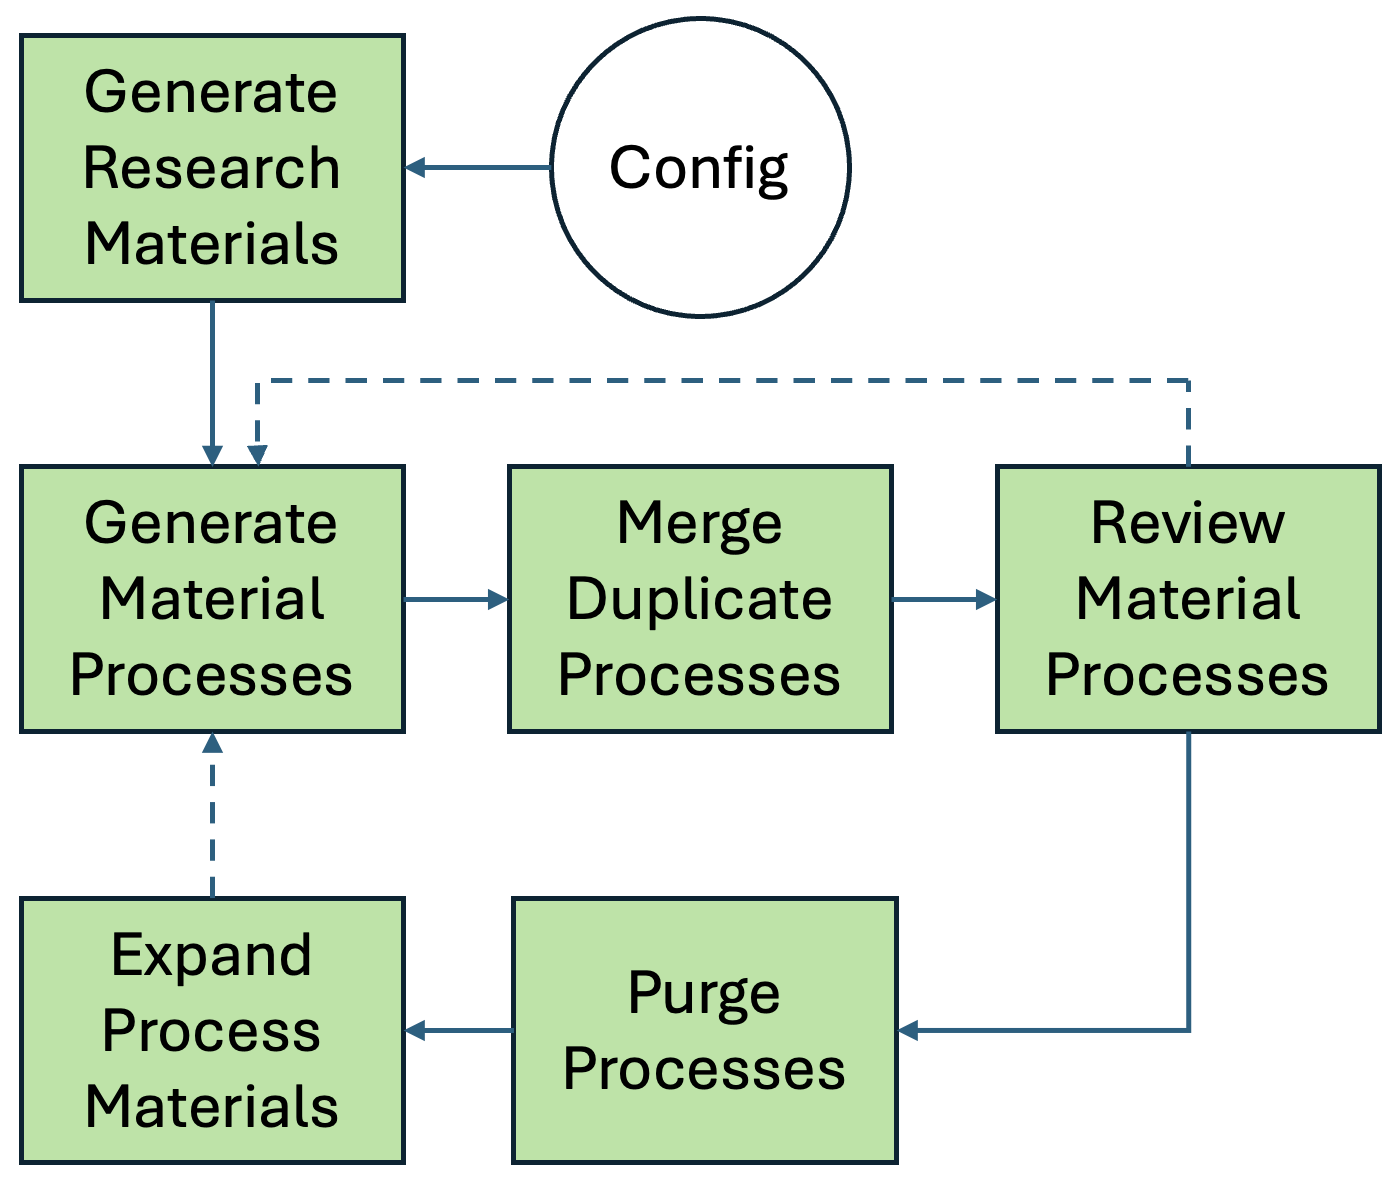
\includegraphics[width=0.9\linewidth]{images/pipeline-tasks2.png}
    \caption{Pipeline Tasks for the multi-agent system.  All tasks, with the exception of the Purge Processes task, use one or more LLM Agents to perform their tasks. }
    \label{fig:pipeline}
\end{figure}

%\subsubsection{System Process Overview: Bottom-Up Material Evolution Graph (MEG) Pipeline Algorithm}
%\mlwcomment{Why have a subsubsection here when it is the only subsubsection? Do we anticipate having more subsubsections, or would it be acceptable to just incorporate this into subsection 3.7?}
%\adscomment{Because the rest got moved to the Appendix. Good catch!}

\iffalse
The system process overview algorithm implements a bottom-up approach for constructing \toolname{} (\tool{}s) that map relationships between materials and manufacturing processes. The pipeline initializes a state object tracking materials, processes, and configuration parameters, with resumption capability from saved progress, then follows an iterative expansion strategy that first generates materials from seed inputs and enters a main loop, alternately discovering new manufacturing processes for existing materials and identifying additional upstream/downstream materials to support those processes. The algorithm employs a purging mechanism to remove processes lacking sufficient material support, ensuring realistic network dependencies. It continues to expand until reaching the maximum number of iterations or user termination, returning a directed hypergraph where the vertices represent the materials and the hyperedges represent the manufacturing processes that connect the input materials to the output products.
\fi

Lower-level algorithm breakdowns for Material Generation and Review, Process Generation and Merge, Review Processes, Purge Processes, and Upstream/Downstream Expansion are detailed in Appendix A.

\subsubsection{Material Generation}
Material generation initiates the pipeline, beginning with seed materials specified through the command-line interface. A \textbf{material classification agent} utilizes a large language model to analyze industrial contexts, chemical taxonomies, and harmonized trade nomenclatures, identifying materials that function as direct intermediates derived from existing nodes or downstream products positioned along the transformation chain. For each newly identified material, the agent extracts its canonical name, corresponding six-digit Harmonized System (HS) code, mined status indicating natural occurrence (ore, brine, mineral compound) versus refined/intermediate classification, aliases encompassing chemical synonyms and trade names, primary downstream applications, and formal HS description for standardized classification. This process operates iteratively, with each discovered material layer serving as input for subsequent generation rounds. Through multiple iterations, the method constructs a hierarchical node structure spanning naturally occurring forms, intermediate compounds, and advanced products.

\subsubsection{Process Generation and Merging}

Process generation constitutes the primary mechanism for network expansion beyond material nodes. A \textbf{manufacturing process agent} examines each material node to identify industrial transformations that either produce or consume the material. For processes that produce the material, the agent traces upstream manufacturing steps and input requirements. For processes that consume the material, the agent identifies downstream transformation pathways and resulting products. Each discovered process is recorded as a \textbf{hyperedge} containing a descriptive narrative of the transformation, scale designation (industrial, commercial, or laboratory), explicit lists of precursors and products linked by HS codes, and supporting references retrieved from web sources, technical reports, patents, and other documentation. The process generation task iterates across all material nodes to ensure comprehensive process discovery, with new processes introducing additional upstream or downstream materials that feed back into the material generation phase for continued network expansion.

Network growth produces multiple hyperedges that may describe identical processes with variations in descriptive language or reference sources. The process merging task addresses this redundancy by comparing all edges and identifying those with matching input and output material sets. When duplicate processes are detected, they are consolidated into a single canonical hyperedge that combines all supporting references from the original edges. This merging operation maintains network compactness and interpretability while preventing artificial inflation of the edge set through redundant process descriptions. A separate \textbf{reference review agent} evaluates the quality and reliability of supporting documentation later in the pipeline, ensuring the iterative approach between process generation and material generation drives systematic construction of the technology dependency network.

\subsection{Integration of External Tools and Data}

The system incorporates several external data sources and tools that are accessible to LLM agents during network construction. These components are integrated through the Model Context Protocol:

\begin{itemize}
    \item \textbf{HS Code MCP Tool} -- Provides semantic search capabilities for standardized six-digit harmonized system codes and assigns trade classifications to materials.
    \item \textbf{Reference cache vector store} -- Maintains previously retrieved documents and supports semantic search for reuse of existing evidence and references.
    \item \textbf{Web search MCP Tool} -- Enables agents to access external online sources for identification of new supporting documents.
    \item \textbf{Wikipedia MCP Tool} -- Supplies structured encyclopedic data on materials and processes for initial discovery tasks.
\end{itemize}

These tools provide access to both standardized classification data and current reference material, supporting evidence-based network construction and validation.

\subsection{User Interaction via CLI}
User interaction with the system is managed through a \textbf{command-line interface (CLI)} that provides control over network construction and inspection functions. The CLI supports \textbf{material seeding}, allowing users to initialize the pipeline with one or more starting materials. \textbf{Task execution} functions enable users to run individual pipeline components or initiate the complete iterative workflow. The interface includes \textbf{network inspection} capabilities for reviewing materials, processes, and their associated references at any stage of development. Additionally, \textbf{reference management} functions allow users to update data sources, refresh cached information, or manually incorporate external documentation.

This design accommodates both single-session exploratory analysis and extended network development projects where the material evolution graph is constructed and refined over multiple sessions.

\section{Experimental Results/Evaluation}
\label{sec:experiments}


% The Material Evolution Graph is implemented as a directed hypergraph to represent industrial transformations and material dependencies.
% \anil{structural properties: degree distribution of nodes, reachability of individual products}


\subsection{Implementation details}

Using our approach, we produced four separate \tool{}s for Germanium, Gallium, Cobalt, and Boron. For each, we started with a material or family of related materials (for example, Cobalt starts with three different related materials - see Table 1). For each, common materials were identified (within the realm of microelectronics) that require the starting material for their production. Lastly, all transformation processes necessary to produce these materials were discovered (see Table 1). Due to the time required for each iteration, the material and process identification phases for creating these four hypergraphs were limited to five iterations.

\begin{table}[h!]
\centering
{\small
\begin{tabularx}{8.5cm}{|>{\raggedright\arraybackslash}p{3.5cm}|X|X|}
\hline
\footnotesize\textbf{Starting Material(s)\newline [Node(s)] } & \footnotesize\textbf{Transformation\newline Materials\newline [Nodes]} & \footnotesize\textbf{Transformation\newline Processes\newline [Hyperedges]} \\
\hline
Germanium & 59 & 59 \\
\hline
Gallium & 89 & 79 \\
\hline
Cobalt (cobalt ore, cobalt mattes, cobalt oxide) & 65 & 66 \\
\hline
Boron (boric acid, borax, sodium borate, boron carbide, borane, boron trifluoride, boron compounds) & 84 & 61 \\
\hline
\end{tabularx}
}
\caption{\tool{} sizes (node and hyperedge counts) for each starting material.}
\label{tab:transformations}
\end{table}

% \begin{figure}
%     \centering
% 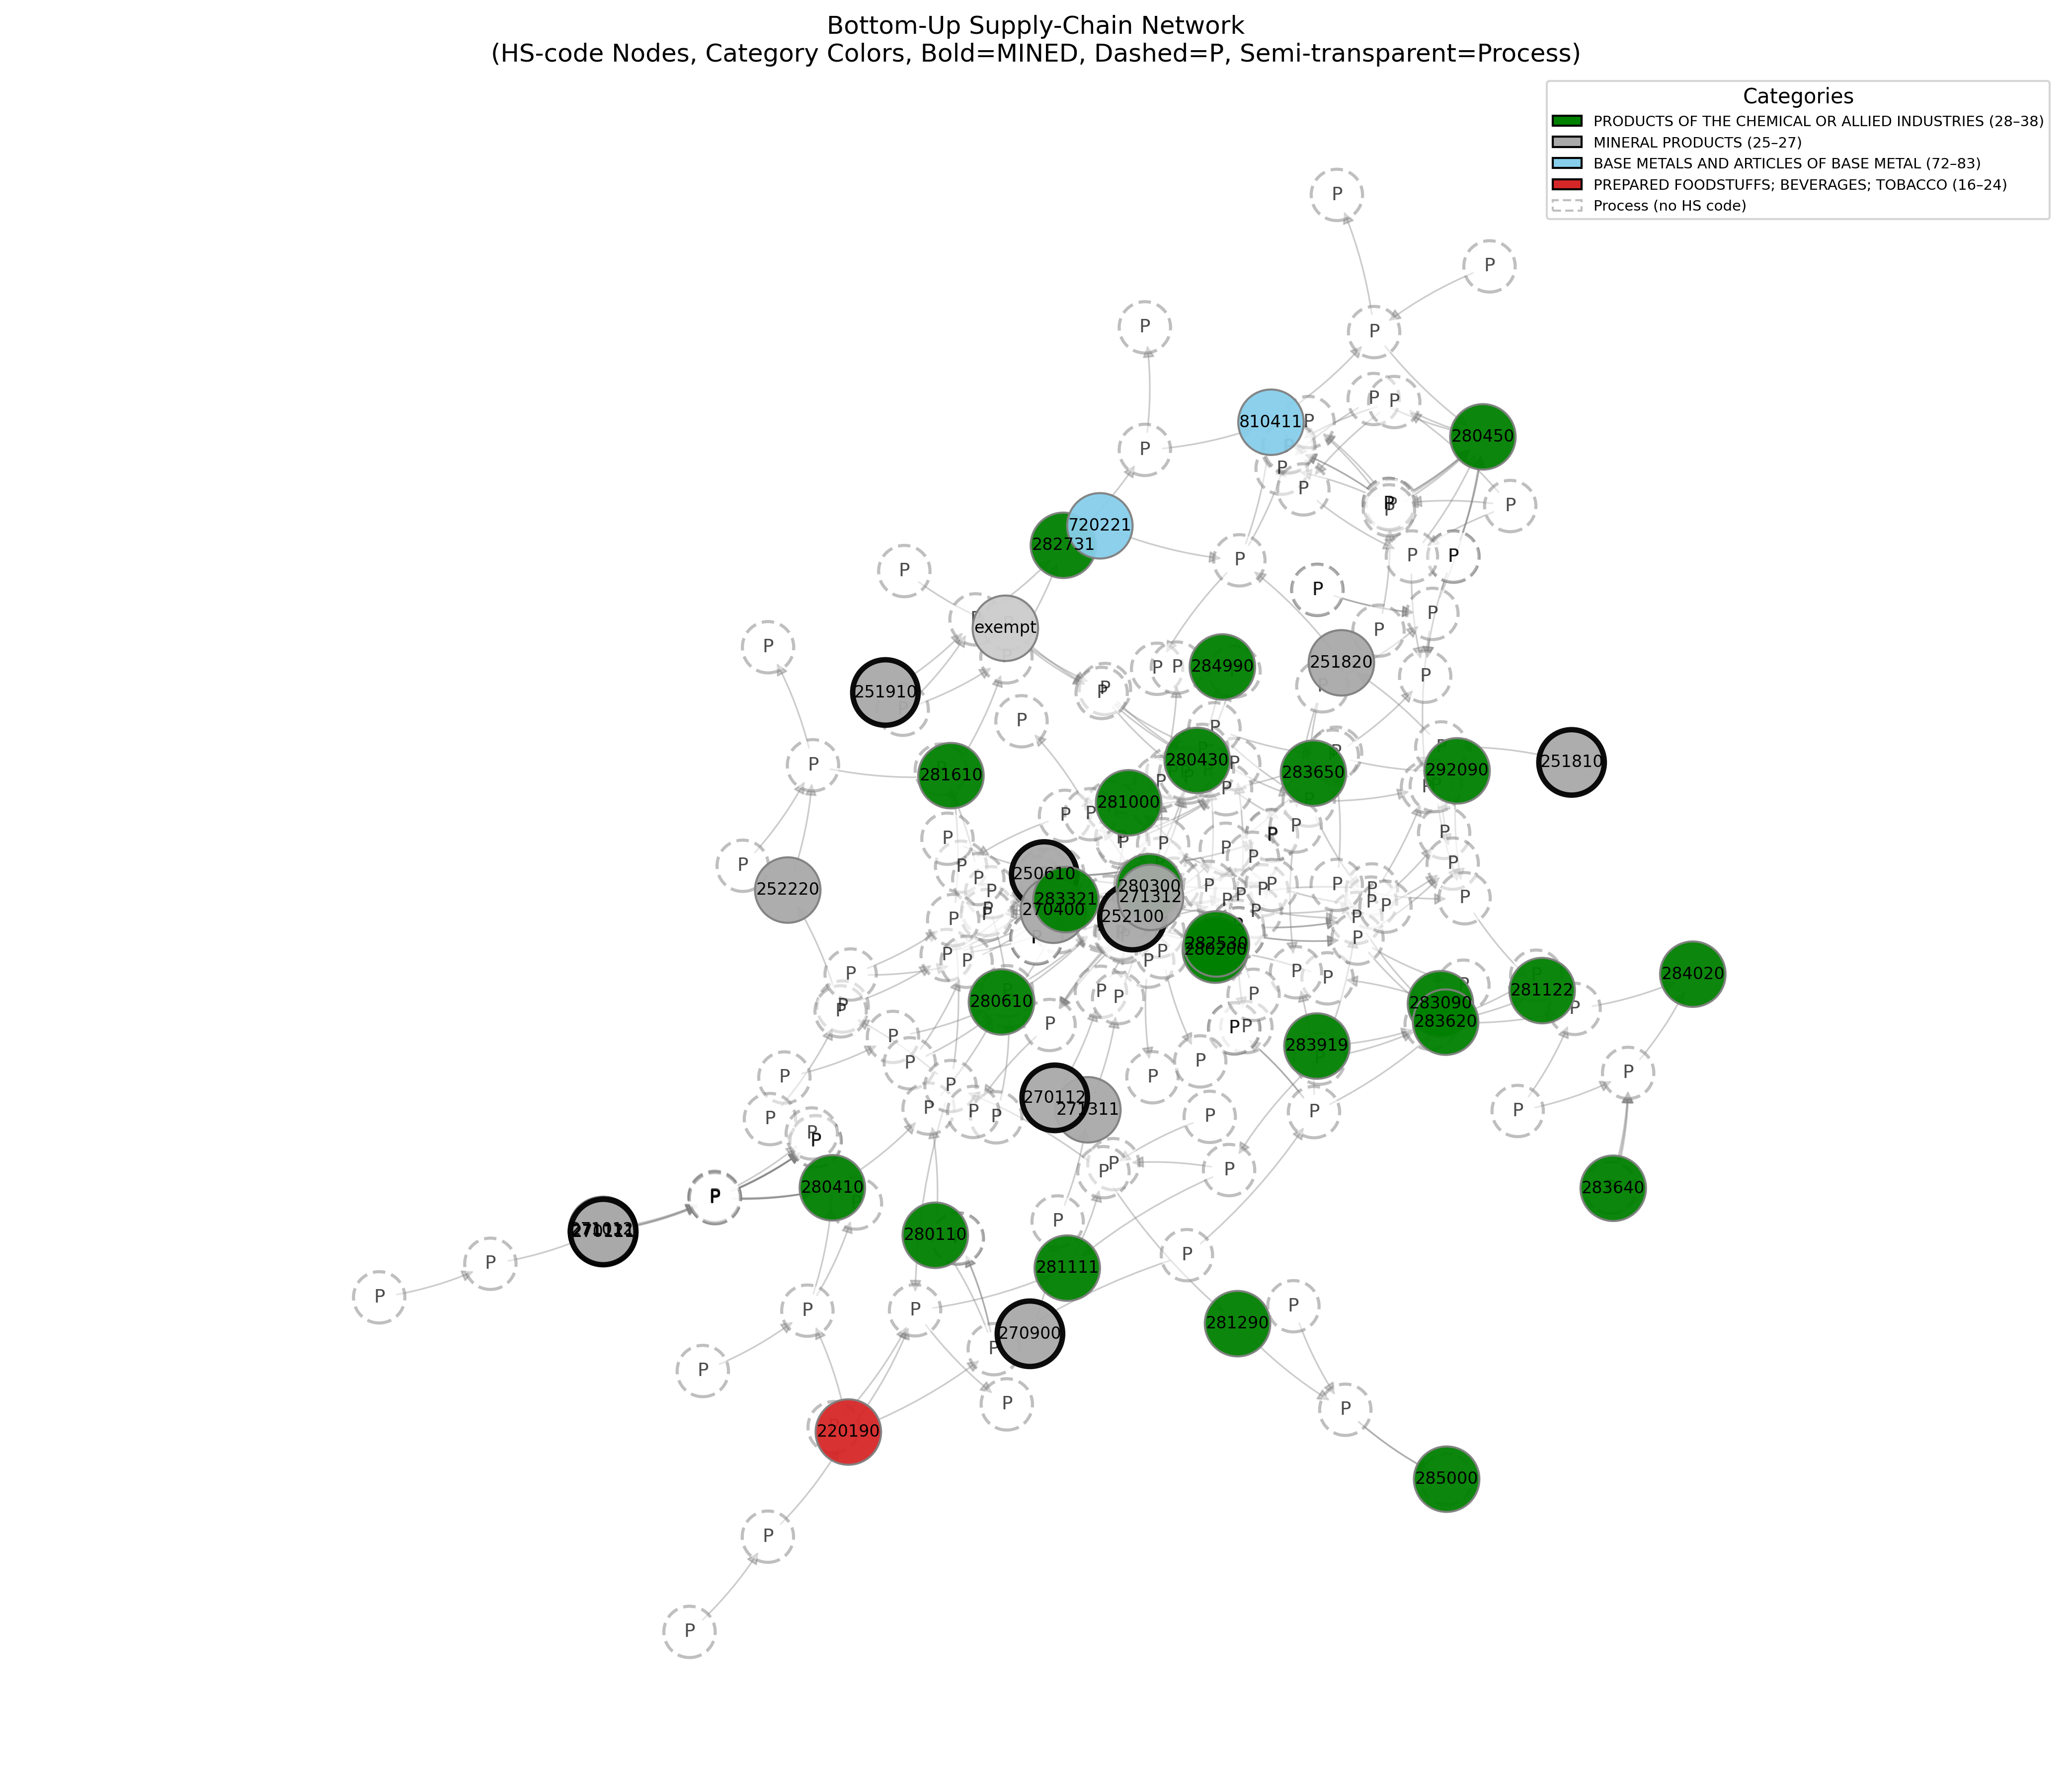
\includegraphics[width=1.0\linewidth]{images/network_analysis_network.png}
% \caption{Directed Projection of \tool{} for Boron. } 
% \label{fig:Boron-viz}
% \end{figure}


\begin{figure}[h]
    \centering
    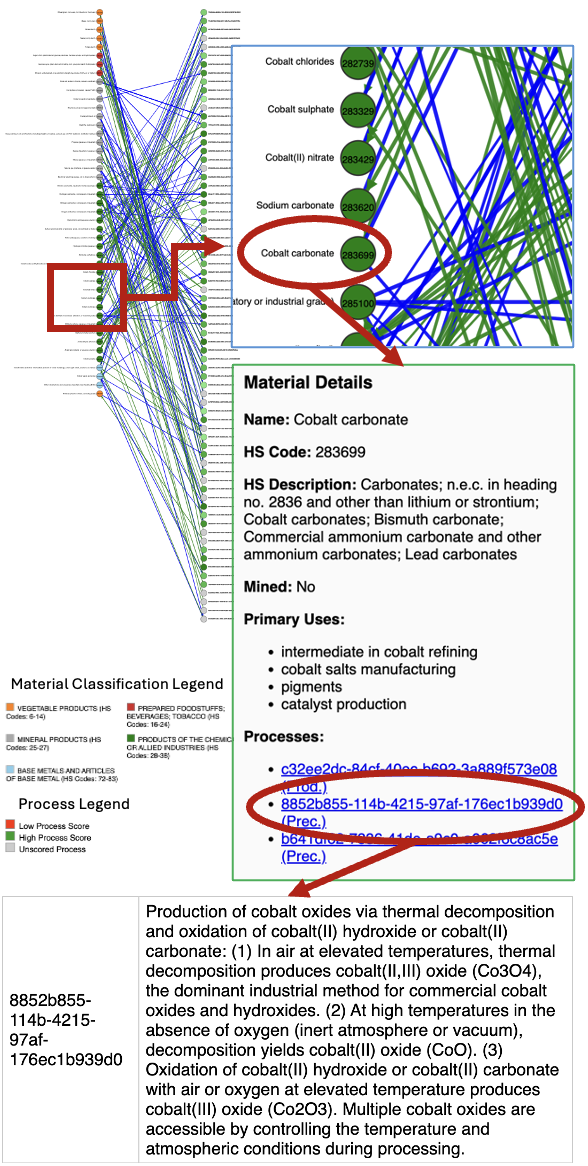
\includegraphics[width=0.9\linewidth]{images/bottom-up-vis-3.png}
    \caption{Network Graph Visualization and Interaction.  Material Nodes (left) are shown connected to one or more process hyperedges (right). Blue lines show the inputs to the processes.  Green lines show the outputs of the process.}
    \label{fig:netgraph-details}
\end{figure}

Using the generated vertices and hyperedges, a hypergraph was constructed for each material. 
Figure~\ref{fig:netgraph-details} shows a visualization of the generated hypergraph for Boron. The hypergraph $\Hcal(M,E)$ is visualized as a directed bipartite graph $G(V_1, V_2, E_G)$ with the materials as the nodes on the left and the processes (hyperedges in the original hypergraph) as the nodes on the right. For each material $m \in M$, we introduce a node $v_m \in V_1$ in $G$. For each hyperedge $e = (e_s, e_t) \in E$, we introduce a node $v_e \in V_2$ in $G$. For every material in the source
set of $e$, i.e., for each $m \in e_s$, we add a directed edge $(v_m, v_e)$ to $E_G$. Similarly, for every material in the target
set of $e$, i.e., for each $m \in e_t$, we add a directed edge $(v_e, v_m)$ to $E_G$. The visualization also zooms in on a few
nodes to show details.
% Figures \ref{fig:Boron-viz} and \ref{fig:netgraph-details} show two different visualizations of the generated hypergraphs for Boron. Figure \ref{fig:Boron-viz}, a directed projection of the multi-hypergraph,  is a simplified graph derived from the full directed hypergraph representation of the material processing network. In the original hypergraph, each process connects multiple precursor materials (inputs) to one or more product materials (outputs). The directed projection translates that structure into a standard directed graph, where edges represent directional relationships between entities—either from a material to the process that consumes it (precursor → process) or from a process to the material it produces (process → product). This projection makes it possible to apply conventional network-analysis methods (such as degree, reachability, and centrality) while still preserving the directionality and flow of transformations across materials and processes.  Figure \ref{fig:netgraph-details} presents an alternative visualization, where the material nodes are represented on the left and the processes (hyperedges) are represented as nodes on the right.  The lines between them represent precursor and product links between the two.


% $\Hcal(M, E)$, each $e=(A, B)\in E$

% $R(S) = \cup_T{\mbox{there is a sequence of hyper edges from $S$ to $T$}}$

% $(A, B), (B, C), $

% $R(v) = \cup_{S, v\in S} R(S)$

\subsubsection{Vertices (Nodes): Materials}

Each vertex/node represents a distinct material and contains the following data: a \textbf{canonical name} that provides standardized identification, a \textbf{six-digit HS code} for global trade classification, and a \textbf{mined status} flag indicating whether the material is extracted from natural sources or represents an intermediate compound. Additional attributes include \textbf{aliases} for alternative names and trade designations, \textbf{primary downstream uses} describing industrial applications, and the \textbf{HS code description} providing the official classification text. This node structure connects materials across industrial domains, trade categories, and chemical classification systems. Figure \ref{fig:netgraph-details} shows an example of what a material node looks like under Material Details. 

\subsubsection{Hyperedges: Transformation Processes}

Transformation processes are represented as hyperedges that link multiple input materials to multiple output materials. Each hyperedge contains a \textbf{descriptive narrative} of the transformation process, \textbf{scale information} indicating industrial, commercial, or laboratory operation, and \textbf{precursor and product lists} linked to material nodes via HS codes. Associated references include \textbf{URLs}, \textbf{source quality scores} reflecting domain credibility, \textbf{content relevance scores} indicating process support, and a derived \textbf{process confidence score}. Hyperedges with identical input and output HS code sets are de-duplicated while retaining all supporting references.

\subsection{Structural Analysis}
\label{sec:criticality}
% \subsubsection{Traceability and Connectivity}

\begin{figure}
    \centering
% 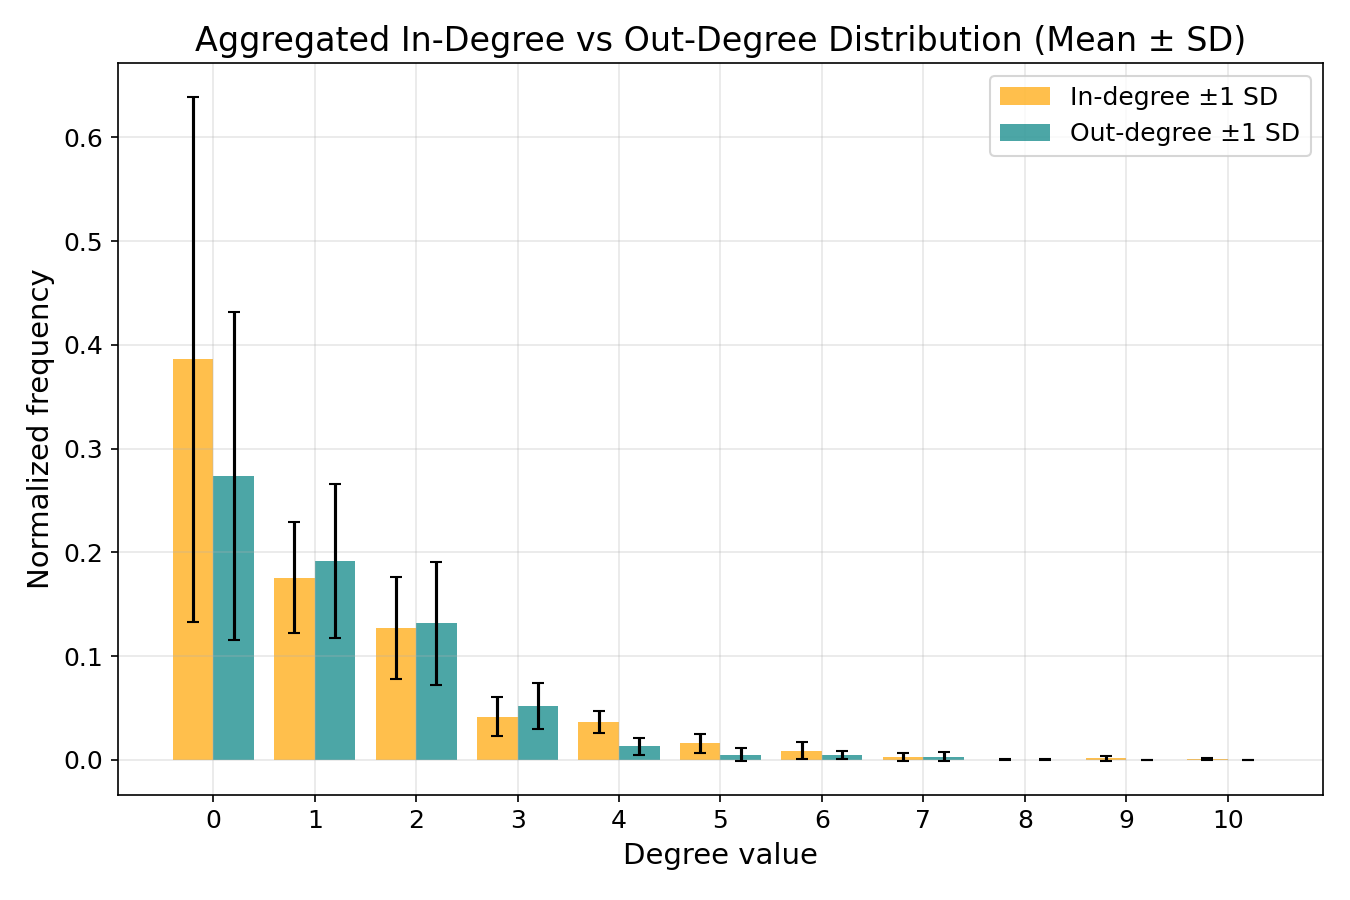
\includegraphics[width=0.9\linewidth]{images/summary_degree_comparison_avgdist.png}
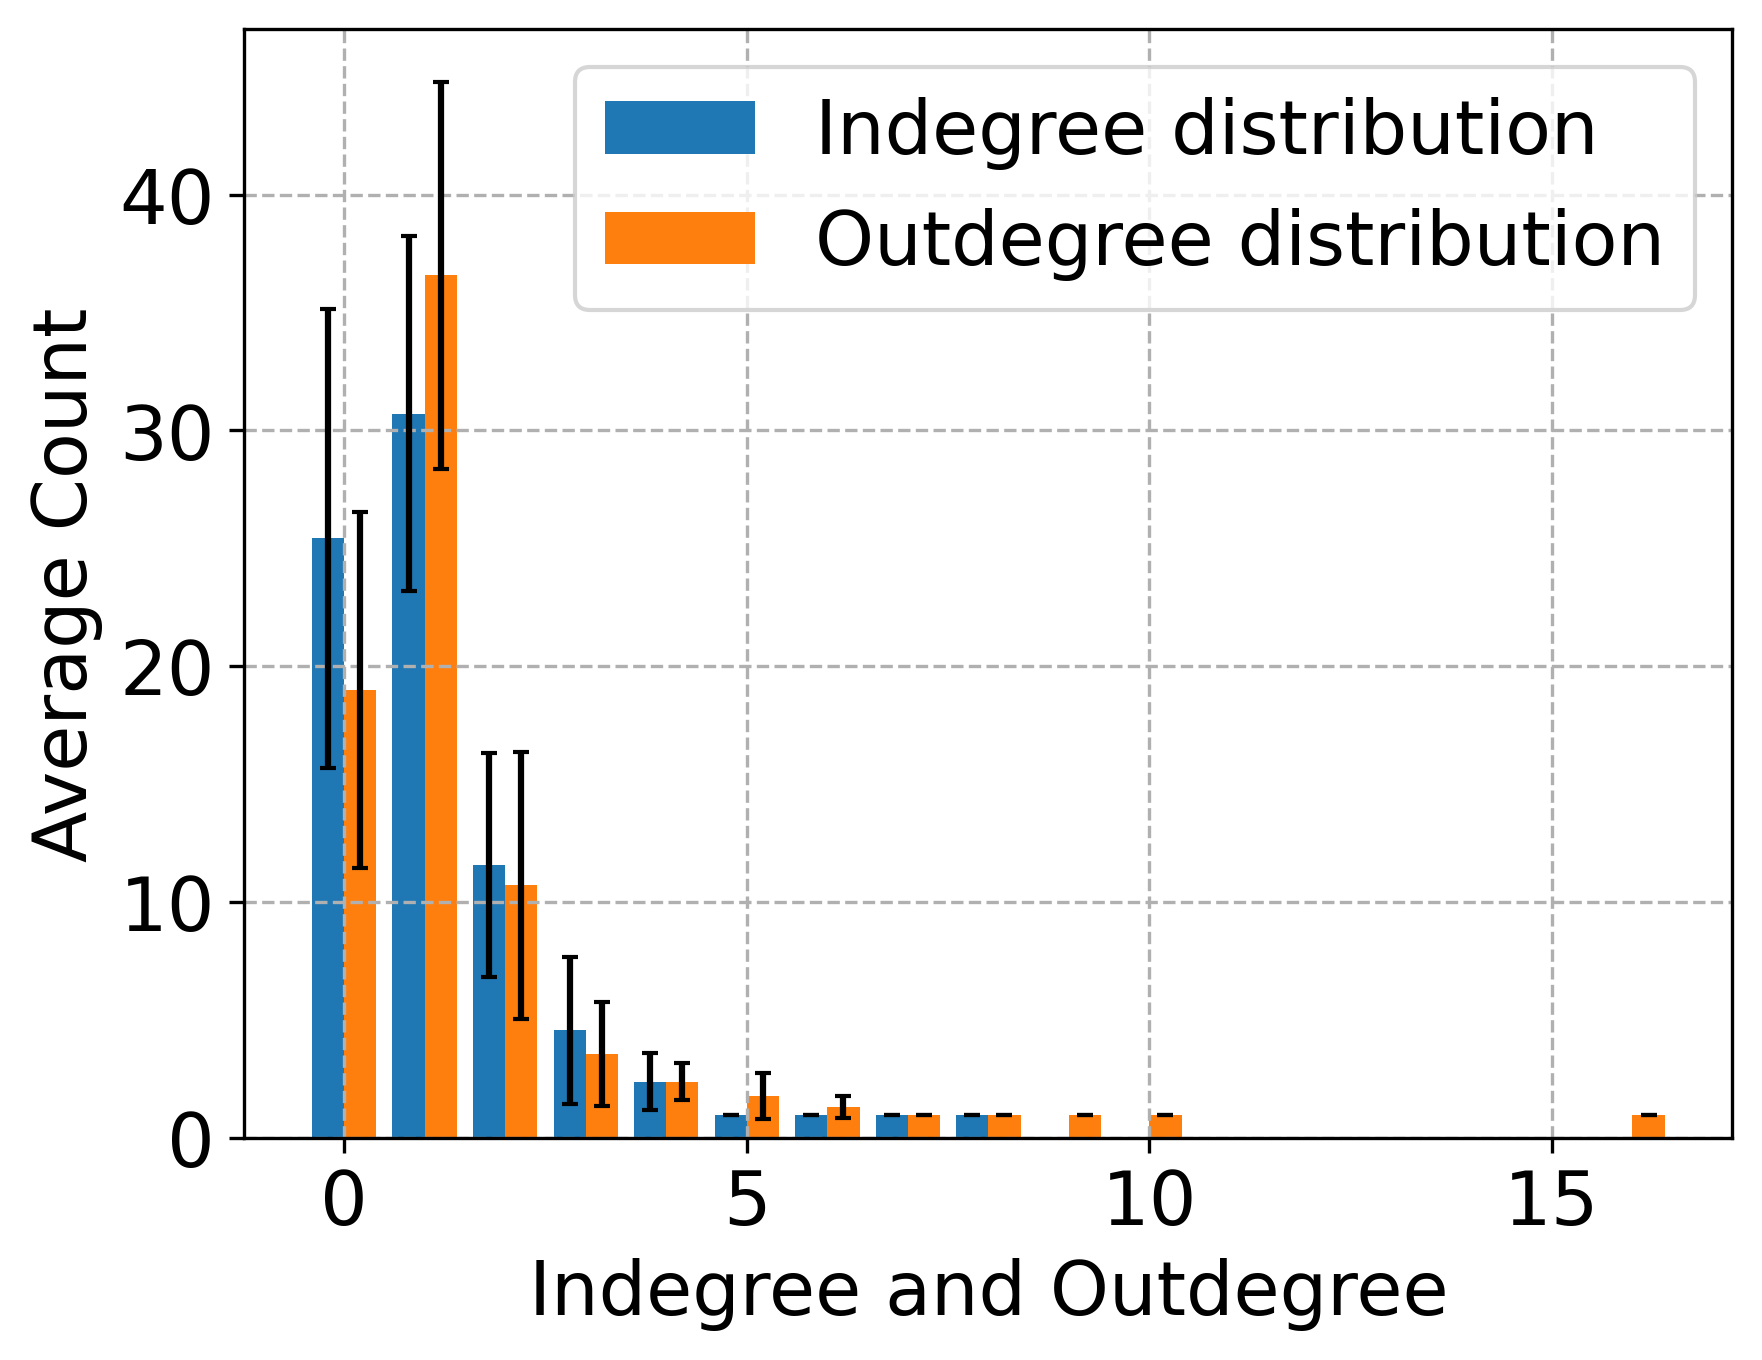
\includegraphics[width=0.9\linewidth]{images/boron_degree_distributions.png}
\caption{In- and Out-degree distributions of \tool{} for Boron, computed from 7 independently generated instances. Error bars show one standard deviation.}
\label{fig:degree}
\end{figure}


We analyze some of the fundamental network properties of the \tool{}s for Boron.
% degree, reachability and centrality distributions.
% High values with respect to these metrics can indicate high criticality for these processes. 
The most basic metric is the degree distribution.
For a node $v\in M$, we define the out-degree $d_{out}(v)=|\{e=(e_s, e_t)\in E: v\in e_s\}|$ as the number of hyperedges for which it is part of the source.
Similarly, we define the in-degree $d_{in}(v)=|\{e=(e_s, e_t)\in E: v\in e_t\}|$.
Figure~\ref{fig:degree} shows the in- and out-degrees of nodes in \tool{}s for Boron. 
Only a small fraction of nodes are involved in multiple processes, and are critical from that perspective.

The hypergraph structure supports bidirectional traversal: downstream materials can be traced to their mined origins, and extracted materials can be followed to derived intermediates and products. 
The network reveals parallel pathways to identical products, indicating potential substitution routes and alternative production methods. 
Bottleneck processes appear as hyperedges connecting otherwise separate network components. This structure supports both pathway analysis and quantitative assessment of connectivity, redundancy, and material criticality.


% \subsection{Analysis of material criticality}

We now define a notion of criticality for materials that constitute a \tool{}. The intuitive idea is as follows. Each \tool{} is
constructed for a given base material, e.g., Boron, which we denote as $m_{base}$. The \tool{} describes the set of processes (hyperedges) by which $m_{base}$,
in combination with other raw materials, can be used to generate new materials. The total set of materials that can be generated
in this way is the \textit{reach} of $m_{base}$ in the \tool{} hypergraph. The notion of reach is similarly defined for any
material $m \in M$.

The criticality of any other material in the \tool{} is the reduction in the number of materials that can be generated if we
remove this material from the \tool{}. Thus, it is the reduction in the reach of $m_{base}$ when the other material
is removed. From a policy perspective, removing a material could correspond to banning the production and use of that material. 
The impact of the policy is the criticality of the removed material, as it quantifies the cascading effect of removing that 
material on the production of other materials. We formalize these notions below.

\begin{definition}
\label{def:reach}
\textbf{Precursor Set.}
Given a \tool{} $\Hcal(M, E)$, where each hyperedge $e \in E$ has a source set $e_s$ and a target set $e_t$, we define the precursor set $\mathtt{Pre} = \bigcup_e e_s - \bigcup_e e_t$ to be the set of materials which appear only in hyperedge sources.
\end{definition}

\begin{definition}
\label{def:reach}
\textbf{Reachable set.}
Given a \tool{} $\Hcal(M, E)$ and a set $m_{start} \subseteq M$, a material $m_i$ is considered reachable if it is in the
target set of a hyperedge whose source set contains only materials that are in $m_{start}$ or are themselves reachable. The 
reachable set, $R(m_{start}, \Hcal)$ is the set of all nodes that are reachable from $m_{start}$ in $\Hcal$.
\end{definition}

\begin{definition}
\label{def:criticality}
\textbf{Criticality.}
Given a \tool{} $\Hcal(M, E)$ and a set $m_{start} \subseteq M$, the criticality of a material $m_i$ is defined as, 
\begin{align}
\nonumber
c(m_i, m_{start}, \Hcal) = |R(m_{start}, \Hcal)| - |R(m_{start}\setminus m_i, \Hcal \setminus m_i)|,
\end{align}
i.e., it is the reduction in the 
size of the reachable set when $m_i$ is removed.
\end{definition}

In our analysis of criticality, we always set $m_{start} = m_{base} \cup \mathtt{Pre}$. For each \tool{}, we compute $c(m_i, 
m_{start}, \Hcal) \forall m_i \in M$ (except for $m_{base}$ itself). Table~\ref{table:criticality} shows
the top 3 most critical materials for multiple \tool{}s. For a \tool{}, its \textbf{criticality list} is the set $M$ of 
its materials, ordered from most critical to least critical. Note that this list is partially ordered, as several materials can
have the same criticality.

\begin{table}[h]
%\vspace{-0.3in}
%\centering
\caption{Top 3 critical materials in each \tool{}. In each case, $m_{base}$ is written in bold. The criticality value
for $m_{base}$ is $R(m_{base} \cup \mathtt{Pre}, \Hcal)$.}
\begin{center}
% \begin{tabular}{|r|c|} \hline
\begin{tabular}{|R{0.8\linewidth}|l|} \hline
\toprule
Material [HS Code] & Criticality \\ 
\midrule
\textbf{Elemental Boron [284520]} & \textbf{73} \\
Hydrogen (byproduct) [280410] & 12 \\
Oxygen [280440] & 9 \\
Fumed silica [281122] & 8 \\
% Soda Ash (Sodium Carbonate) [283620] & 8 \\
% Silicon tetrachloride [281230] & 7 \\
\midrule
\textbf{Cobalt ore and concentrates [260500]} & \textbf{61} \\
Sodium Chloride (in brine solution) [250100] & 8 \\
Sodium Hydroxide (caustic soda) [281512] & 6 \\
Water (distilled or deionized) [285100] & 5 \\
% Sulfuric acid [280700] & 5 \\
% Hydrogen (elemental, compressed or liquefied) [280410] & 5 \\
\midrule
\textbf{Gallium in ores and concentrates [260600]} & \textbf{53} \\
Lithium bromide [282759] & 7 \\
Lithium chloride [282720] & 6 \\
Carbon monoxide [281121] & 5 \\
% Natural gas [271121] & 5 \\
% Methyllithium [284530] & 4 \\
% \midrule
% \textbf{Quartz (natural silica, silicon ore) [250610]} & \textbf{18} \\
% Silicon (not less than 99\% purity) [280469] & 6 \\
% Sodium silicates [283911] & 5 \\
% Silica sand [250510] & 5 \\
% Silicon dioxide (synthetic silica gel) [281122] & 4 \\
% Ferro-silico-chromium [720250] & 3 \\
\midrule
\textbf{Germanium metal, unwrought [811292]} & \textbf{40} \\
Coke (coal-derived, industrial grade) [270400] & 6 \\
Calcium carbide, industrial grade [284910] & 6 \\
Sawdust or wood shavings [440149] & 5 \\
% Carbon monoxide [282410] & 4 \\
% Lime (Calcium oxide, quicklime) [252210] & 4 \\
\bottomrule
%\hline\end{tabular}
\end{tabular}
\end{center}
\label{table:criticality}
\end{table}

\subsection{Sensitivity Analysis} 
% \samarth{Changed from ``Disruption'' to ``Sensitivity''}

To study the sensitivity of the criticality analysis to the stochasticity in the \tool{} generation process, we
formalize a method for sensitivity analysis. Our approach is quite general, and the criticality analysis can be replaced with 
other kinds of analysis easily.

We assume that a \tool{} $\Hcal(M, E)$ is a sample from an underlying distribution over \tool{}s, $\Phi$. Suppose that we
are interested in computing a function, $F(\Hcal)$, from $\Hcal$, which may be a relevant measure for some policy analysis.
Examples of $F$, based on Section~\ref{sec:criticality}, might be the most critical material, the ordering of the criticality 
list, the distribution of orders in the criticality list (i.e., how many materials are at each level of criticality), etc. We
would like to understand the sensitivity of $F$ to the stochastic variability in the network generation process. We quantify
this as a measure of dispersion of $F$ from its expected value according to $\Phi$. When $F$ is continuous valued, its 
expectation is $E(F) = \sum_\Hcal F(\Hcal)\Phi(\Hcal)$, and sensitivity would be, e.g., its standard deviation $\sigma(F)$ with 
respect to $E(F)$. In practice, since $\Phi$ is unknown, we would use the sample mean, $\overline{F}$, and the sample standard
deviation, $s(F)$.

To generalize this to criticality lists, we use a ranked list aggregation method instead of $\overline{F}$ and a 
measure of agreement over ranked lists instead of $s(F)$. Specifically, we use Borda Count (BC) to generate an
aggregate criticality list, where the score assigned to a list item is its criticality. In the BC method, scores for 
each item are aggregated by summing across lists, and the resulting list is sorted in descending order. For measuring 
the agreement between the aggregate list and each of the individual criticality lists, we use the Rank-biased Overlap 
(RBO)~\cite{webber10rbo} concordance measure.

RBO is an appropriate measure for our application for two reasons: it does not require the lists to have the same lengths or
identical sets of elements, and it allows biasing the measure towards comparing the top-ranked elements through its 
\textit{persistence} parameter (higher values correspond to higher emphasis on the top-ranked elements). Our criticality lists
can have different sets of elements for different samples of the network generated for the same base material. Criticality also
tends to be low for many nodes in the \tool{} and high for relatively few nodes. This is borne out by the distribution of 
criticality scores from the aggregate criticality list shown in Figure~\ref{fig:criticality}. Thus, emphasizing the top-ranked 
elements makes sense. RBO measures the overlap between two lists iteratively at successive depths. Its value ranges from 0 to 
1, where 0 indicates that the lists are disjoint and 1 indicates that they are identical.

We generated seven instances of the Boron \tool{} and computed the criticality list for each of them with $m_{base} = 284520$ 
(elemental boron) in each case. We then used the BC method to construct the aggregate list and computed RBO for each criticality
list with the aggregate list. Persistence was set to 0.98, which corresponds to $\sim50\%$ of the weight being assigned to the top 
35 elements in the lists. The mean value of RBO was 0.462 and its standard deviation was 0.03. This shows that, while the 
criticality lists are not identical, they have good agreement to a significant depth. The low standard deviation shows that all
the criticality lists have about the same overlap with the aggregate list.

\begin{figure}
    \centering
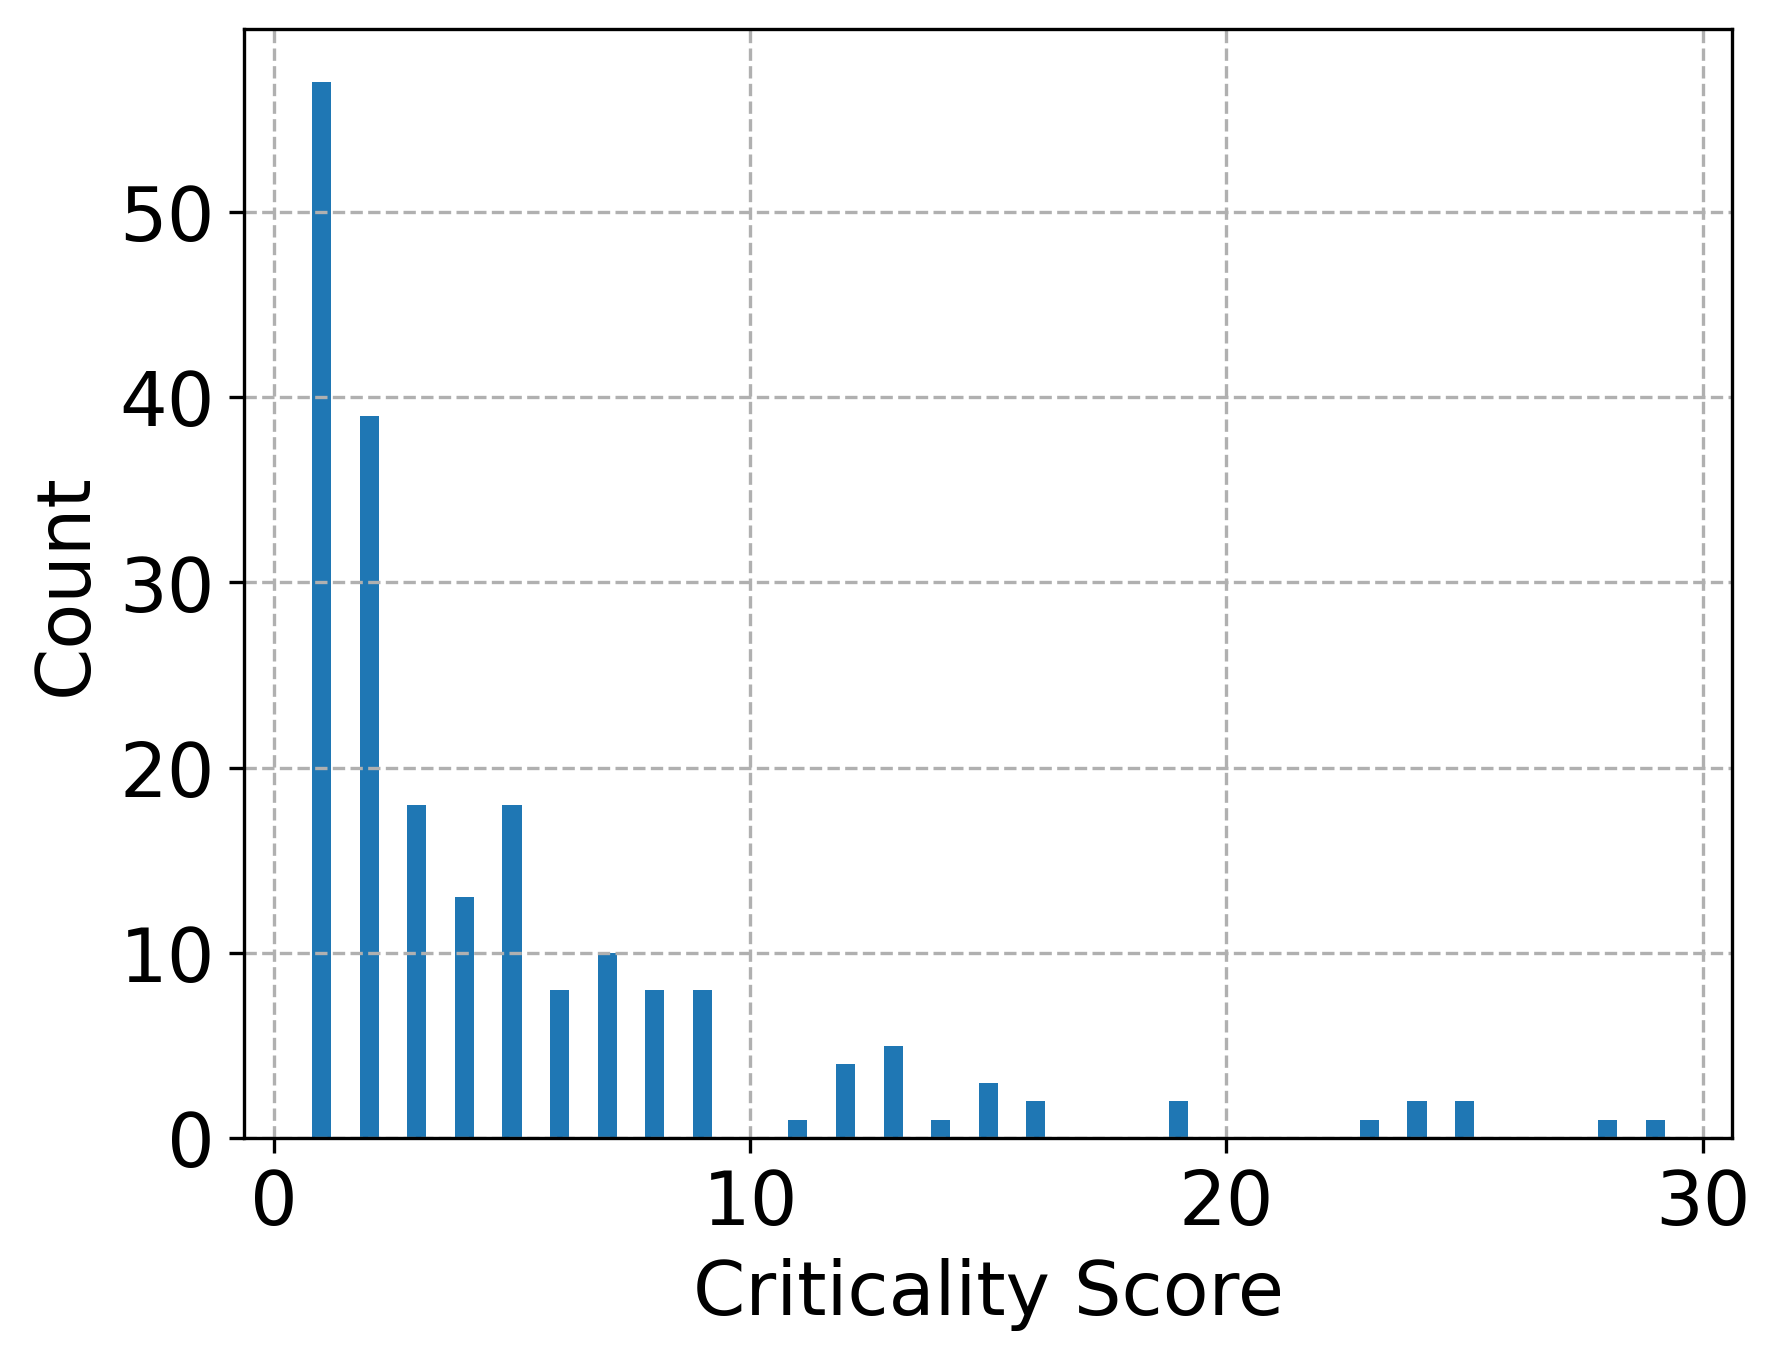
\includegraphics[width=0.9\linewidth]{images/boron_criticality_distribution.png}
\caption{The distribution of criticality scores from the aggregate criticality list for Boron. Note that BC aggregates by summing, so the values here are the sums of the criticalities from the seven criticality lists.}
\label{fig:criticality}
\end{figure}


% In order to study the effects of disruptions on \tool{}s, we present a formalization of disruption analysis.
% This formalization looks specifically at disruptions to \textit{processes} and potential downstream and second-order effects.
% In this model, we additionally endow each material with an availability state $s(m_i) \in [0,1]$, where a fully available material has state $1$, and a fully unavailable material has state $0$.
% We additionally denote by $\varphi(m_i) \subset E$ the set of processes for which $m_i$ is an output, and by $p_{in}$ the set of inputs for process $p$.

% We define a disruption as a flow-based process through the MEG. 
% We update the state of each material according to the following rule.
% For each material $m$, we say that the state of $m$, $s(m) = \max_{p \in \varphi(m)}\min_{m' \in p_{in}}s(m')$. 
% That is to say, each material is disrupted by the process with the least restrictive amount of disruption.
% In this disruption model, we assume that each process is equally capable; that is, if processes $p_1$ and $p_2$ both produce output $m$, they produce equal amounts of $m$. 
% In the initial state, we model a process disruption for process $p$ as setting the state of each $m \in p_{out}$ to be $\frac{|\varphi(m)| - 1}{|\varphi(m)|}$; that is, each output of the process is decreased by the amount created by that output. 

% Because MEGs may have cycles, this update model must propagate through the MEG, until an equilibrium is reached. 
% We say that the equilibrium state is the final disruption analysis, and specifically look at the effect on the material state. 
% \gsh{Open questions: 1. When is an equilibrium guaranteed to exist? 2. Can we efficiently compute the equilibrium state?}


\subsection{Disruption Analysis}
Using the Boron \tool{} and Comtrade data~\cite{UNComtrade2024} for 2024, we
assess how disruptions in countries dominating the export of key raw
or intermediary materials (HS 6-digit level) cascade through
downstream technologies. 
The United Nations Comtrade Database is the official global repository of detailed international trade statistics collected and published by the United Nations. It provides import and export data reported by more than 200 countries and territories, organized by commodity categories and trading partners. The database enables researchers, policymakers, and businesses to analyze global trade flows, economic dependencies, and supply chain dynamics across time and regions.

For each HS 6-digit code in the MEKH, we identify the top supplier using UN Comtrade trade values and apply a 60\% dominance threshold, i.e. the leading exporter must account for at least 60\% of
global exports of that HS code. We then simulate a disruption scenario
in which the dominant supplier halts all exports of that material, and
evaluate the downstream effects on dependent HS codes within the Boron \tool{}. Specifically, any HS codes that rely exclusively on the disrupted
precursor are considered fully removed from the network.

The analysis 
reveals that while disruptions by Mexico (HS 252922),
Norway (271121), Turkey (284011), the United States (284020), and
China (810411) do not propagate further downstream, disruptions by
Poland (HS 280200) and Turkey (HS 284019) cause significant cascading
losses. Specifically, the loss of HS 280200 eliminates five dependent
HS codes, while the disruption of HS 284019 removes
four HS codes. Additionally, the US, which controls 100\% of HS
284520, could disrupt both 284520 and its dependent HS 285000, which
lacks substitute inputs.

Overall, the results indicate that although most disruptions are
localized, a few highly concentrated supply nodes, such as Poland’s HS
280200 and Turkey’s HS 284019, pose significant downstream risks within
the boron \tool{}.

\section{Discussion}
\label{sec:discussion}

There are several recent examples of supply chain vulnerabilities due to shortages in raw and intermediate materials. \tool{}s
are an important means of discovering and exploring such systemic effects.
For example, the COVID-19 pandemic exposed fundamental vulnerabilities in semiconductor supply chains, where hidden intermediates and concentrated manufacturing led to cascading global shortages. Hasan et al.~\cite{hasan2022demand} documented how automotive manufacturers faced severe disruptions because chip suppliers had reallocated production capacity to consumer electronics, revealing how obscured intermediate dependencies amplified supply chain vulnerabilities across multiple industries. The semiconductor shortage demonstrated that traditional top-down visibility failed to capture the complex web of intermediate processing steps and their interdependencies, leading to unexpected bottlenecks~\cite{chakraborty2022empirical,tam2022understanding}.

Similarly, China's dominance in rare earth elements processing illustrates how intermediate transformation stages can create hidden supply chain risks. Zhang et al.~\cite{zhang2024reshaping} found that terbium production in China declined by 90\% between 2007 and 2018, not due to resource scarcity but because existing mining techniques could not meet stringent environmental regulations. This research revealed that only 25\% of China's rare earth production quota was utilized by 2018, indicating that environmental constraints at intermediate processing stages—rather than political restrictions—had become the primary supply bottleneck. The study highlighted how top-down approaches focusing on end products missed critical vulnerabilities in upstream processing capabilities.

The lithium battery supply chain presents another compelling example of hidden intermediate dependencies. Hu et al.~\cite{hu2025technological} demonstrated that technological risks and export controls on advanced battery manufacturing processes can disrupt entire supply networks, with the United States holding 56-79\% of core technological capabilities. Their analysis revealed that restrictions on cathode formulation technologies and intellectual property transfers created bottlenecks affecting downstream battery production across multiple countries, despite abundant lithium ore availability. The lithium battery case shows that proprietary manufacturing processes and technology dependencies create supply chain vulnerabilities that are invisible to traditional backward-tracing approaches.

The disruptions to semiconductor, rare earth, and lithium batteries demonstrate a fundamental limitation of top-down supply chain analysis: the methodology inherently struggles with opacity at multiple levels of the transformation network. Baldwin et al.~\cite{baldwin2023hidden} provided empirical evidence that traditional face-value supply chain analysis significantly underestimates exposure to foreign suppliers due to hidden intermediates, finding that the U.S. vehicle sector's exposure to Chinese industrial inputs was four times higher than indicated by conventional top-down measures. This ``hidden exposure'' stems from the complex spiral of inputs used to make inputs, which remains largely invisible when starting from finished products and working backward through proprietary supplier networks.
\section{Conclusions}
\label{sec:conclusion}

This work presents an agentic bottom-up pipeline for constructing \toolname{}s (\tool), an essential
building block for supply chain networks that document the transformation of raw materials into refined industrial products. In contrast to top-down approaches constrained by supplier network opacity and hidden intermediaries, this pipeline is built on documented processes from publicly available literature, trade databases, and industrial references.

The system integrates \textbf{directed hypergraph modeling} to represent multi-input, multi-output processes, \textbf{LLM-powered reasoning agents} for automated discovery and material classification, \textbf{evidence-backed validation} that scores and removes poorly supported transformations, and \textbf{iterative expansion mechanisms} that identify upstream gaps and extend toward target product categories. These components work together to construct networks with verifiable traceability to source documentation.

The framework facilitates the identification of process bottlenecks, alternative production pathways, and material dependencies crucial for supply chain analysis and critical mineral assessment. The reference cache and accumulated knowledge from previous iterations inform subsequent network expansion and validation cycles, improving the accuracy and completeness of the constructed networks over time.

\section{Code and Data Availability}

The software is available via an anonymized repository for review: \url{https://anonymous.4open.science/r/lia-B773}.

%%%%%%%%%%%%%%%%%%%%%%%%%%%%%%%%%%%%%%%%%%%%%%%%%%%%%%%%%%%%%%%%%%%%%%%%



%%% The acknowledgments section is defined using the "acks" environment
%%% (rather than an unnumbered section). The use of this environment
%%% ensures the proper identification of the section in the article
%%% metadata as well as the consistent spelling of the heading.

\begin{acks}
\end{acks}



%%%%%%%%%%%%%%%%%%%%%%%%%%%%%%%%%%%%%%%%%%%%%%%%%%%%%%%%%%%%%%%%%%%%%%%%

%%% The next two lines define, first, the bibliography style to be
%%% applied, and, second, the bibliography file to be used.

\bibliographystyle{ACM-Reference-Format}
\bibliography{references}

%%%%%%%%%%%%%%%%%%%%%%%%%%%%%%%%%%%%%%%%%%%%%%%%%%%%%%%%%%%%%%%%%%%%%%%%

\clearpage


\end{document}
